\section{戴逊级数}

\subsection{自能}

有了图形表示后,重要的是对图形进行分类。可以使用各种各样的标准对图形进行分类。比如按考虑相互作用的阶数进行分类:

\begin{eqnarray*}
i G (x,x') & = & \left\langle \Phi_0 \right| T \left( \psi(x) \psi^\dagger (x') S \right) \left| \Phi_0  \right\rangle_c \\
{} & = & i G^{(0)} + iG^{(1)} + iG^{(2)} + ... 
\end{eqnarray*}

对$i G^{(1)}$,有两个图:

\begin{equation*}
G^{(1)}(k) = G_a^{(1)} (k) + G_b^{(1)} (k) = G^{(0)}(k) \Sigma^{(1)}(k) G^{(0)}(k)
\end{equation*}

这里的$\Sigma^{(1)}(k)$叫一阶自能:

\begin{equation}
\Sigma^{(1)}(k) = \frac{i}{(2 \pi)^4 } \int d^4p e^{i p_0 \eta} \left( V(k-p) G^{(0)}(p)  - V(0) G^{(0)}(p)  \right) 
\end{equation}

按照这个思路还可以考虑二阶自能$\Sigma^{(2)}(k) $,即包含两根相互作用线的自能图。

对二阶自能图,可分成两类,一类是切断一根单粒子线,自能图就能分成独立的两部分,每一部分分别是个一阶自能图:

\begin{equation*}
\Sigma^{(1)} G^{(0)}  \Sigma^{(1)}
\end{equation*}

还有一类,是不能通过切断一根单粒子线分成不相连两部分的。这部分是真正不同于一阶图形的部分,我们称之为正规自能。当然这里是二阶的正规自能$\Sigma^{(2)*}$。

我们可以把各阶的正规自能都加在一起,得到作为整体的正规自能$\Sigma^*$。

\begin{equation}
\Sigma^* = \Sigma^{(1)*} + \Sigma^{(2)*} + ...
\end{equation}

自能$\Sigma$可表示为:

\begin{equation}
\Sigma = \Sigma^* + \Sigma^* G^{(0)} \Sigma^* + \Sigma^* G^{(0)} \Sigma^* G^{(0)} \Sigma^* + ...
\end{equation}

这是一种对图形的分类,即正规自能,通过一根单粒子线连接起的两个正规自能,通过两根单粒子线连接起的三个正规自能……,这种分类方式并不遗漏,也不重复。

将格林函数用自能$\Sigma (k)$表示,

\begin{equation}
G(k) = G^{(0)}(k) + G^{(0)}(k) \Sigma(k) G^{(0)}(k)
\end{equation}

将格林函数用正规自能$\Sigma^* (k)$表示,

\begin{equation}
G(k) = G^{(0)}(k) + G^{(0)}(k) \Sigma^* (k) G(k)
\end{equation}

把$G(k)$都挪到左边:

\begin{equation*}
G(k) \left( 1 - G^{(0)} (k) \Sigma^* (k)  \right) = G^{(0)}(k)  
\end{equation*}

注意:这里的$G$,$G^0$,$\Sigma^* $都是$c$数,

\begin{equation*}
G^{-1} = \left( G^{(0)} \right)^{-1} \left( 1 - \Sigma^*  G^{(0)}  \right) = \left( G^{(0)} \right)^{-1} - \Sigma^*
\end{equation*}

这意味着:

\begin{equation}
G(k) = \frac{1}{  \left( G^{(0)} (k) \right)^{-1} - \Sigma^* (k)  }
\end{equation}

正规自能的实部是对准粒子能量的修正,而正规自能的虚部是对准粒子寿命的修正。考虑相互作用后格林函数的求解被归结为对正规自能的求解。

\subsection{一阶自能}

作为例子,我们来计算$\Sigma^{(1)}(k)$,先计算积分:

\begin{equation}
\frac{-i}{(2 \pi)^4} \int d^4 p V(0) G^{(0)}(p) e^{i p_0 \eta}
\end{equation}

改写为:

\begin{equation*}
-i \int \frac{d^3 p}{(2 \pi)^3} \int \frac{ d \omega }{ 2 \pi } V(0) \left( \frac{\theta(p - p_F)}{ \omega - \epsilon_p + i \eta } + \frac{ \theta(p_F - p) }{ \omega - \epsilon_p - i \eta }    \right) e^{i \omega \eta}
\end{equation*}

对$e^{i \omega \eta}$,积分回路取上半平面,沿大圆的积分为0。

\begin{equation*}
\oint ... = \int_{- \infty}^{\infty} ... = 2 \pi i (Rez (\omega = \epsilon_p + i \eta)) = 2 \pi i \frac{ \theta(p_F - p) }{2 \pi} = i \theta(p_F - p)
\end{equation*}

考虑:$\int d^3 x \int \frac{d^3 p}{(2 \pi)^3} ... = V \int \frac{d^3 p}{(2 \pi)^3} ... = N $

\begin{equation*}
-i \int \frac{d^3 p}{(2 \pi)^3} ... = - i \cdot i \frac{N}{V} V(0)= n V(0) 
\end{equation*}

类似地,计算积分,

\begin{equation*}
i \int \frac{d^3 p}{(2 \pi)^3 } \int \frac{ d \omega }{ 2 \pi } e^{i \omega \eta } V(k-p) \left(  \frac{\theta(p-p_F)}{ \omega - \epsilon_p + i \eta}  + \frac{ \theta(p_F -p)  }{ \omega - \epsilon_p - i \eta }     \right)
\end{equation*}

先利用留数定理对$\omega$积分,

\begin{equation*}
 - \int \frac{d^3 p}{(2 \pi)^3 } V(k-p) \theta(p_F - p)
\end{equation*}

得到$\Sigma^{(1)}(k)$的表达式:

\begin{equation}
\Sigma^{(1)}(k) = n V(0) - \frac{1}{(2 \pi)^3} \int d^3 p V ( \vec k - \vec p ) \theta( p_F - | \vec p | )
\end{equation}

考虑$\Sigma^{(1)}(k)$的近似是超出普通的微扰论的,因为在公式$G^{-1} = \left( G^{(0)} \right)^{-1} - \Sigma^* $里已经考虑了很多诸如$\Sigma^1 G^0 \Sigma^1$,$\Sigma^1 G^0 \Sigma^1 G^0 \Sigma^1$...的近似。

\subsection{极化}

\begin{equation*}
U(q) = V(q)  + V(q) \Pi(q) V(q)
\end{equation*}

这里$V$表示裸相互作用线,$U$表示考虑了多体效应后的相互作用线。我们称$\Pi(q) $为极化。

\begin{figure}[htbp]
\begin{center}
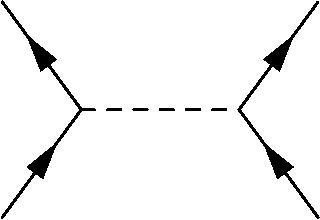
\includegraphics[width=5cm]{Zero/polarized.png}
\caption{裸相互作用线,我们可以在裸相互作用线里不断插入“泡泡”图。}
%\label{default}
\end{center}
\end{figure}

类似于自能,我们把极化分为两类,正规极化$\Pi^*$,和非正规极化$\Pi_{ir}$,正规极化是无法通过切断一根裸相互作用线而把极化分为两个不连接的两部分的极化图形。

极化$\Pi$可以用正规极化$\Pi^*$来表示:

\begin{equation}
\Pi = \Pi^* + \Pi^* V \Pi^* + \Pi^* V \Pi^* V \Pi^* + ... 
\end{equation}

考虑极化后的相互作用线$U$,可以用正规极化$\Pi^*$来表示:

\begin{equation}
U = V + V \Pi^* U
\end{equation}

或改写为:

\begin{equation*}
U (1 - \Pi^* V) = V
\end{equation*}

即:

\begin{eqnarray*}
U(q)  & = &  \frac{V(q)}{1 - \Pi^*(q) V(q) } = \frac{V(q)}{\epsilon(q)} \\
{} & = & V(q) ( 1 + \Pi^* (q) V (q) + \Pi^* (q) V (q) \Pi^* (q) V (q) + ...  )
\end{eqnarray*}

这里:$\epsilon(q) = 1 - \Pi^*(q) V(q) $
